\section{BTB\_\-2levbtac\_\-t Class Reference}
\label{classBTB__2levbtac__t}\index{BTB\_\-2levbtac\_\-t@{BTB\_\-2levbtac\_\-t}}
Inheritance diagram for BTB\_\-2levbtac\_\-t:\nopagebreak
\begin{figure}[H]
\begin{center}
\leavevmode
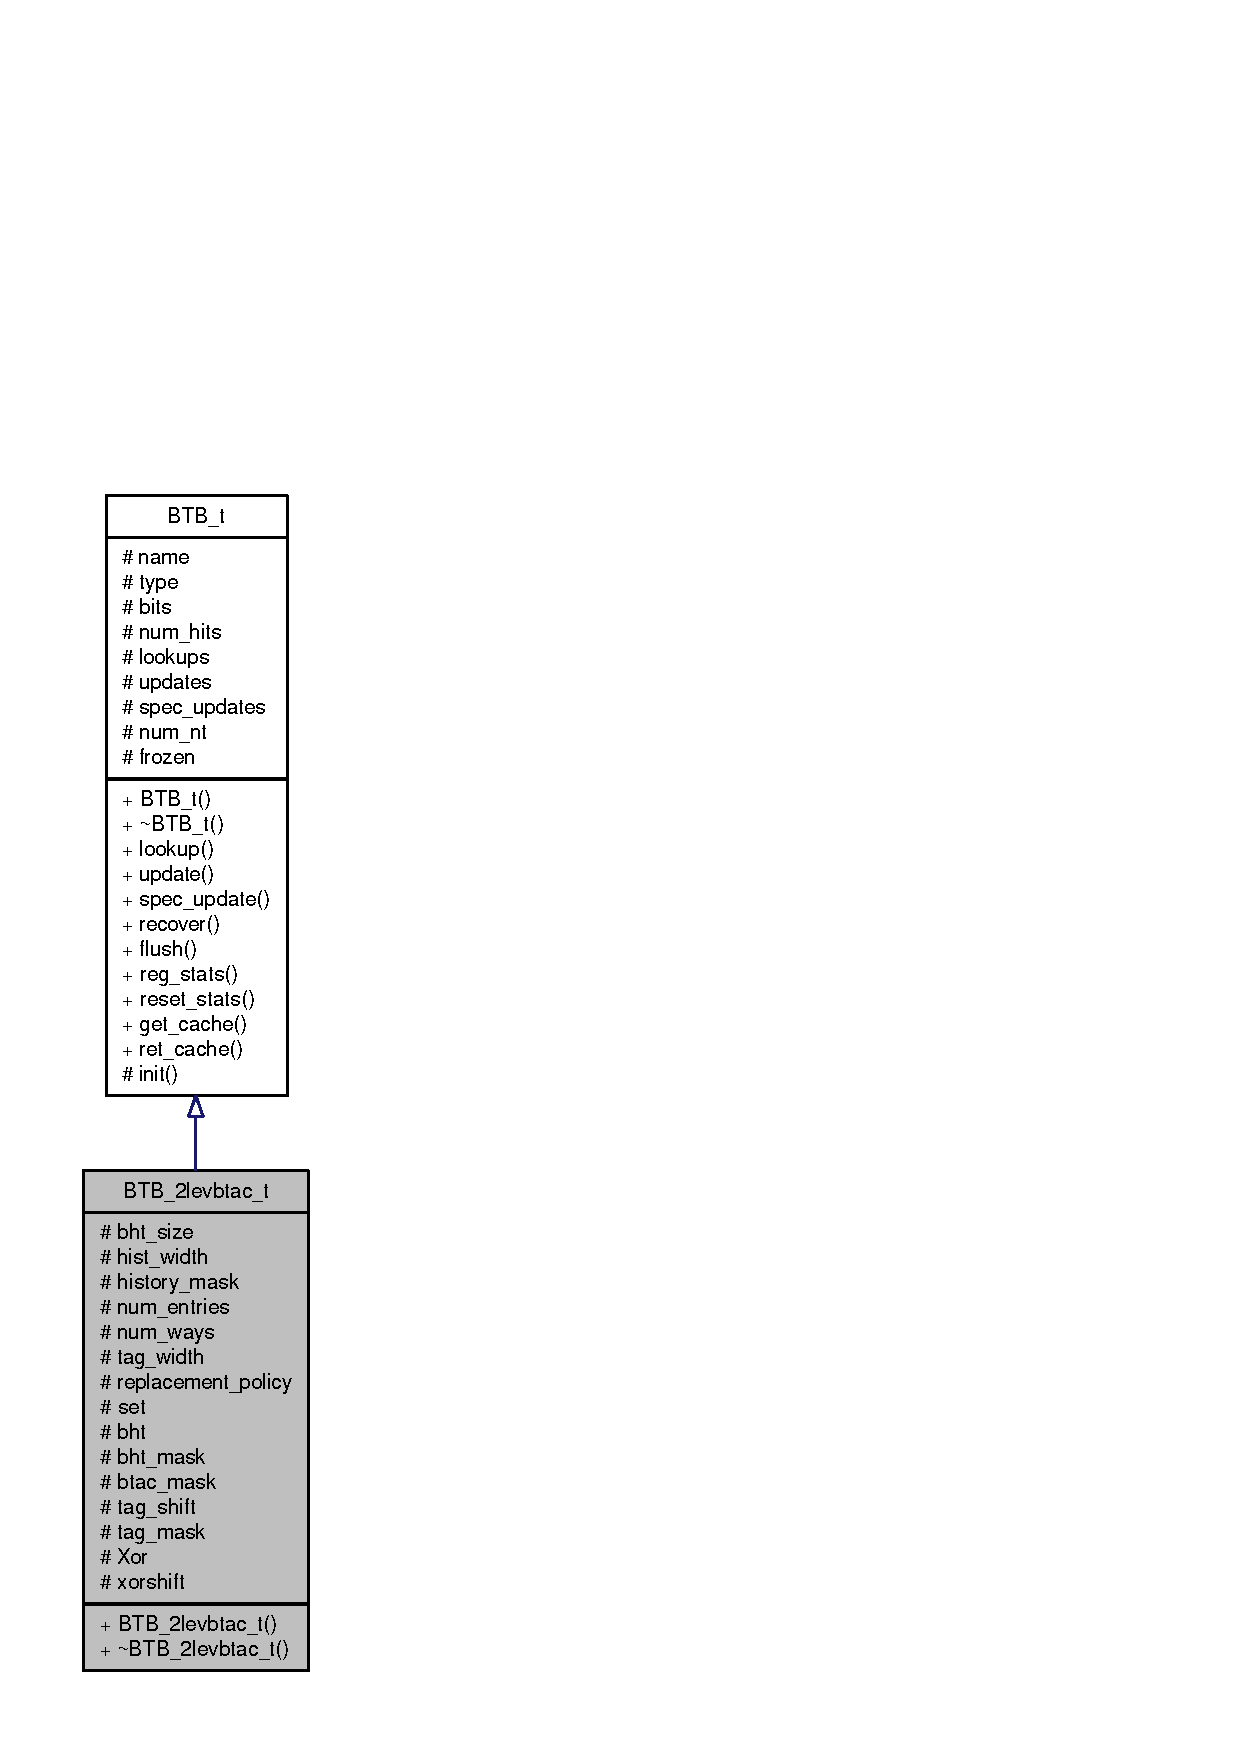
\includegraphics[height=400pt]{classBTB__2levbtac__t__inherit__graph}
\end{center}
\end{figure}
Collaboration diagram for BTB\_\-2levbtac\_\-t:\nopagebreak
\begin{figure}[H]
\begin{center}
\leavevmode
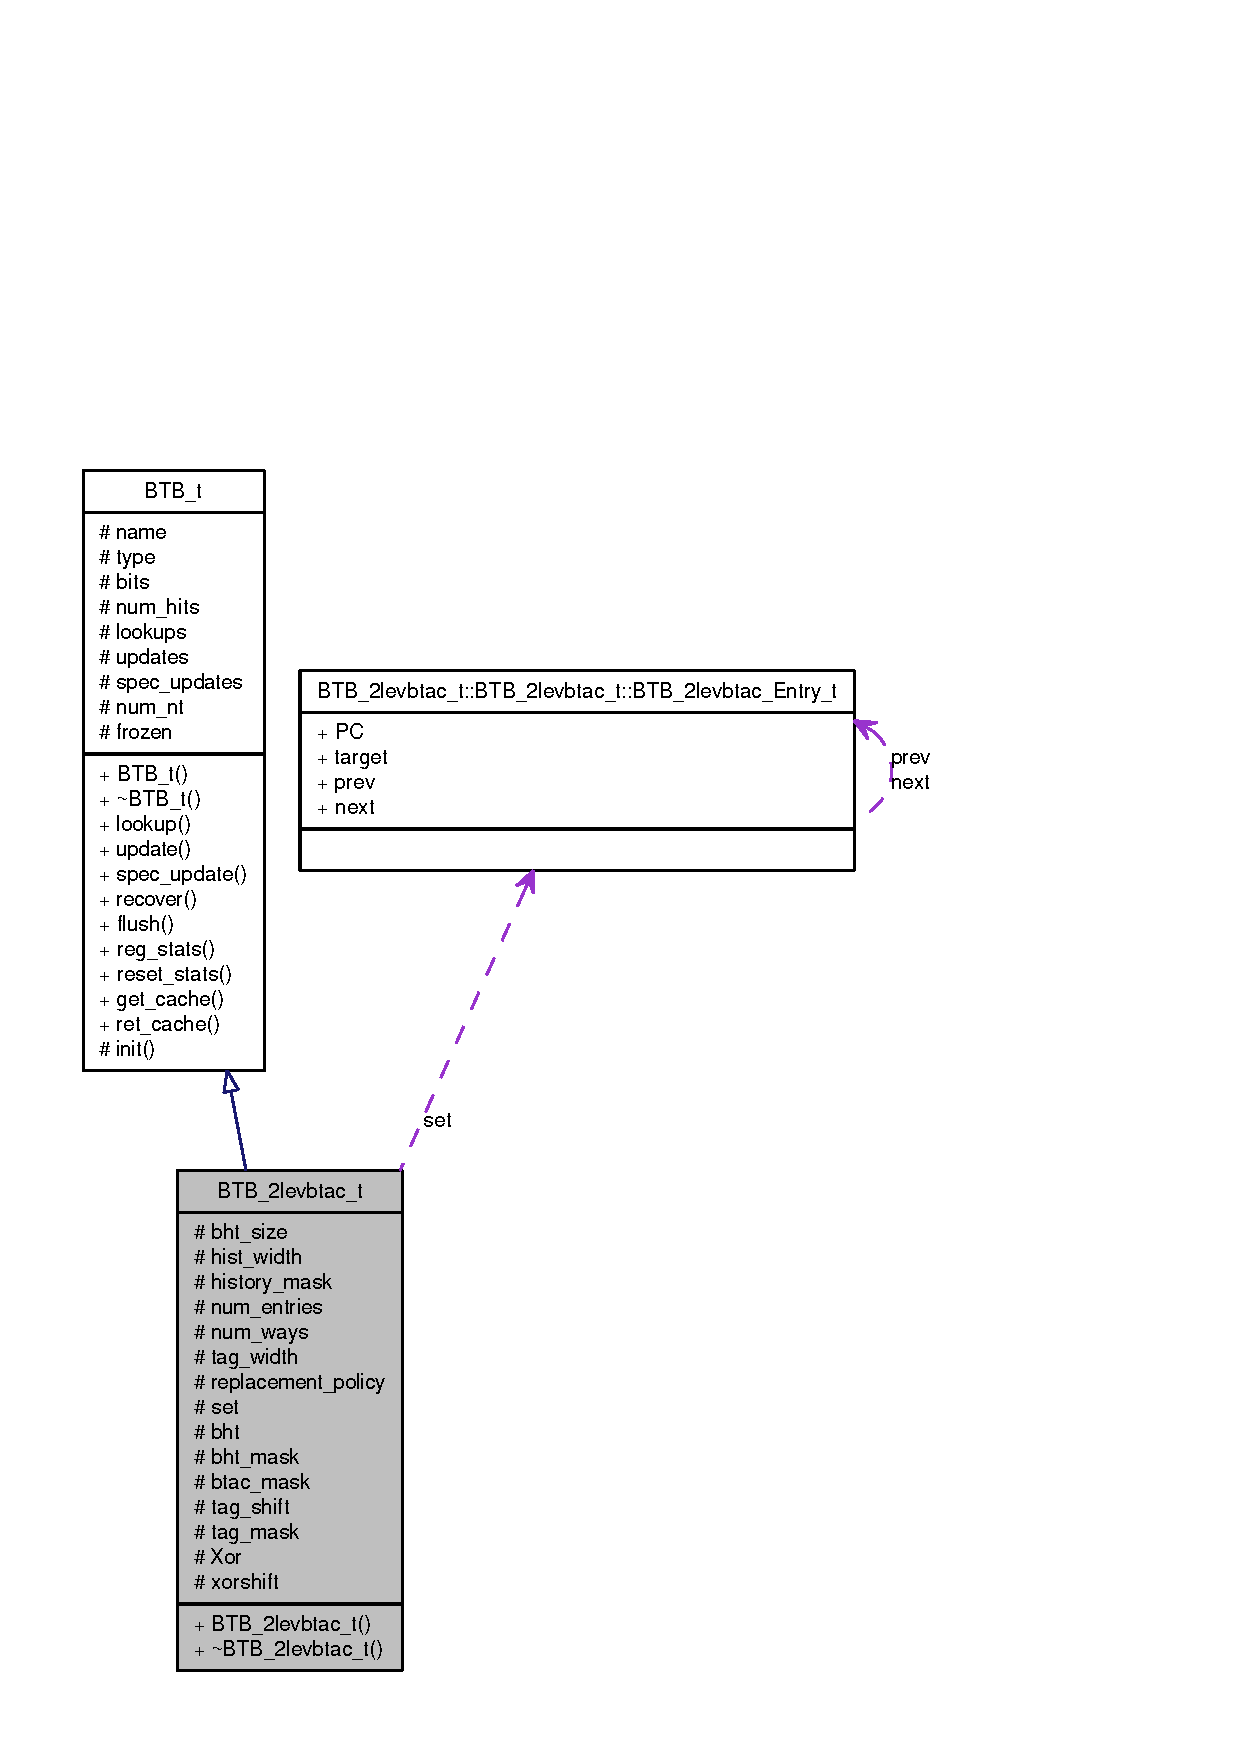
\includegraphics[width=400pt]{classBTB__2levbtac__t__coll__graph}
\end{center}
\end{figure}
\subsection*{Classes}
\begin{CompactItemize}
\item 
struct {\bf BTB\_\-2levbtac\_\-Entry\_\-t}
\item 
class {\bf BTB\_\-2levbtac\_\-sc\_\-t}
\end{CompactItemize}
\subsection*{Public Member Functions}
\begin{CompactItemize}
\item 
{\bf BTB\_\-2levbtac\_\-t} (char $\ast$const arg\_\-name, const int arg\_\-bht\_\-size, const int arg\_\-hist\_\-width, const int arg\_\-Xor, const int arg\_\-num\_\-entries, const int arg\_\-num\_\-ways, const int arg\_\-tag\_\-width, const char arg\_\-replacement\_\-policy)
\item 
{\bf $\sim$BTB\_\-2levbtac\_\-t} ()
\end{CompactItemize}
\subsection*{Protected Attributes}
\begin{CompactItemize}
\item 
int {\bf bht\_\-size}
\item 
int {\bf hist\_\-width}
\item 
int {\bf history\_\-mask}
\item 
int {\bf num\_\-entries}
\item 
int {\bf num\_\-ways}
\item 
int {\bf tag\_\-width}
\item 
char {\bf replacement\_\-policy}
\item 
struct {\bf BTB\_\-2levbtac\_\-Entry\_\-t} $\ast$$\ast$ {\bf set}
\item 
int $\ast$ {\bf bht}
\item 
int {\bf bht\_\-mask}
\item 
int {\bf btac\_\-mask}
\item 
int {\bf tag\_\-shift}
\item 
int {\bf tag\_\-mask}
\item 
int {\bf Xor}
\item 
int {\bf xorshift}
\end{CompactItemize}


\subsection{Detailed Description}


Definition at line 24 of file btb-2levbtac.cpp.

\subsection{Constructor \& Destructor Documentation}
\index{BTB\_\-2levbtac\_\-t@{BTB\_\-2levbtac\_\-t}!BTB\_\-2levbtac\_\-t@{BTB\_\-2levbtac\_\-t}}
\index{BTB\_\-2levbtac\_\-t@{BTB\_\-2levbtac\_\-t}!BTB_2levbtac_t@{BTB\_\-2levbtac\_\-t}}
\subsubsection[{BTB\_\-2levbtac\_\-t}]{\setlength{\rightskip}{0pt plus 5cm}BTB\_\-2levbtac\_\-t::BTB\_\-2levbtac\_\-t (char $\ast$const  {\em arg\_\-name}, \/  const int {\em arg\_\-bht\_\-size}, \/  const int {\em arg\_\-hist\_\-width}, \/  const int {\em arg\_\-Xor}, \/  const int {\em arg\_\-num\_\-entries}, \/  const int {\em arg\_\-num\_\-ways}, \/  const int {\em arg\_\-tag\_\-width}, \/  const char {\em arg\_\-replacement\_\-policy})\hspace{0.3cm}{\tt  [inline]}}\label{classBTB__2levbtac__t_36e2ee0f27bd59b849b73400c6a146a2}




Definition at line 70 of file btb-2levbtac.cpp.

References bht, bht\_\-mask, bht\_\-size, BTB\_\-t::bits, btac\_\-mask, CHECK\_\-BOOL, CHECK\_\-POS, CHECK\_\-PPOW2, COMPONENT\_\-NAME, fatal(), hist\_\-width, history\_\-mask, BTB\_\-t::init(), log\_\-base2(), mytolower(), BTB\_\-t::name, BTB\_\-2levbtac\_\-t::BTB\_\-2levbtac\_\-t::BTB\_\-2levbtac\_\-Entry\_\-t::next, num\_\-entries, num\_\-ways, BTB\_\-2levbtac\_\-t::BTB\_\-2levbtac\_\-t::BTB\_\-2levbtac\_\-Entry\_\-t::prev, replacement\_\-policy, tag\_\-mask, tag\_\-shift, tag\_\-width, BTB\_\-t::type, Xor, and xorshift.\index{BTB\_\-2levbtac\_\-t@{BTB\_\-2levbtac\_\-t}!$\sim$BTB\_\-2levbtac\_\-t@{$\sim$BTB\_\-2levbtac\_\-t}}
\index{$\sim$BTB\_\-2levbtac\_\-t@{$\sim$BTB\_\-2levbtac\_\-t}!BTB_2levbtac_t@{BTB\_\-2levbtac\_\-t}}
\subsubsection[{$\sim$BTB\_\-2levbtac\_\-t}]{\setlength{\rightskip}{0pt plus 5cm}BTB\_\-2levbtac\_\-t::$\sim$BTB\_\-2levbtac\_\-t ()\hspace{0.3cm}{\tt  [inline]}}\label{classBTB__2levbtac__t_7e49390d90ecb67a003aac4a28efc90b}




Definition at line 154 of file btb-2levbtac.cpp.

References bht, BTB\_\-t::name, BTB\_\-2levbtac\_\-t::BTB\_\-2levbtac\_\-t::BTB\_\-2levbtac\_\-Entry\_\-t::next, num\_\-entries, and BTB\_\-t::type.

\subsection{Member Data Documentation}
\index{BTB\_\-2levbtac\_\-t@{BTB\_\-2levbtac\_\-t}!bht@{bht}}
\index{bht@{bht}!BTB_2levbtac_t@{BTB\_\-2levbtac\_\-t}}
\subsubsection[{bht}]{\setlength{\rightskip}{0pt plus 5cm}int$\ast$ {\bf BTB\_\-2levbtac\_\-t::bht}\hspace{0.3cm}{\tt  [protected]}}\label{classBTB__2levbtac__t_09ea0fd8512c3b89db1e84c28fc19d26}




Definition at line 55 of file btb-2levbtac.cpp.

Referenced by BTB\_\-2levbtac\_\-t(), and $\sim$BTB\_\-2levbtac\_\-t().\index{BTB\_\-2levbtac\_\-t@{BTB\_\-2levbtac\_\-t}!bht\_\-mask@{bht\_\-mask}}
\index{bht\_\-mask@{bht\_\-mask}!BTB_2levbtac_t@{BTB\_\-2levbtac\_\-t}}
\subsubsection[{bht\_\-mask}]{\setlength{\rightskip}{0pt plus 5cm}int {\bf BTB\_\-2levbtac\_\-t::bht\_\-mask}\hspace{0.3cm}{\tt  [protected]}}\label{classBTB__2levbtac__t_daaef5d4082038f3c40b6cd212cb7d3d}




Definition at line 57 of file btb-2levbtac.cpp.

Referenced by BTB\_\-2levbtac\_\-t().\index{BTB\_\-2levbtac\_\-t@{BTB\_\-2levbtac\_\-t}!bht\_\-size@{bht\_\-size}}
\index{bht\_\-size@{bht\_\-size}!BTB_2levbtac_t@{BTB\_\-2levbtac\_\-t}}
\subsubsection[{bht\_\-size}]{\setlength{\rightskip}{0pt plus 5cm}int {\bf BTB\_\-2levbtac\_\-t::bht\_\-size}\hspace{0.3cm}{\tt  [protected]}}\label{classBTB__2levbtac__t_50ae5ed21b27ecdb87912e1a3adcc911}




Definition at line 47 of file btb-2levbtac.cpp.

Referenced by BTB\_\-2levbtac\_\-t().\index{BTB\_\-2levbtac\_\-t@{BTB\_\-2levbtac\_\-t}!btac\_\-mask@{btac\_\-mask}}
\index{btac\_\-mask@{btac\_\-mask}!BTB_2levbtac_t@{BTB\_\-2levbtac\_\-t}}
\subsubsection[{btac\_\-mask}]{\setlength{\rightskip}{0pt plus 5cm}int {\bf BTB\_\-2levbtac\_\-t::btac\_\-mask}\hspace{0.3cm}{\tt  [protected]}}\label{classBTB__2levbtac__t_795c92f669b0671db88d666304b0cf1c}




Definition at line 58 of file btb-2levbtac.cpp.

Referenced by BTB\_\-2levbtac\_\-t().\index{BTB\_\-2levbtac\_\-t@{BTB\_\-2levbtac\_\-t}!hist\_\-width@{hist\_\-width}}
\index{hist\_\-width@{hist\_\-width}!BTB_2levbtac_t@{BTB\_\-2levbtac\_\-t}}
\subsubsection[{hist\_\-width}]{\setlength{\rightskip}{0pt plus 5cm}int {\bf BTB\_\-2levbtac\_\-t::hist\_\-width}\hspace{0.3cm}{\tt  [protected]}}\label{classBTB__2levbtac__t_27f4c02daffbdf13ffe9e3e88bac997c}




Definition at line 48 of file btb-2levbtac.cpp.

Referenced by BTB\_\-2levbtac\_\-t().\index{BTB\_\-2levbtac\_\-t@{BTB\_\-2levbtac\_\-t}!history\_\-mask@{history\_\-mask}}
\index{history\_\-mask@{history\_\-mask}!BTB_2levbtac_t@{BTB\_\-2levbtac\_\-t}}
\subsubsection[{history\_\-mask}]{\setlength{\rightskip}{0pt plus 5cm}int {\bf BTB\_\-2levbtac\_\-t::history\_\-mask}\hspace{0.3cm}{\tt  [protected]}}\label{classBTB__2levbtac__t_3d3adf1cba01e21f75d7652a777c140c}




Definition at line 49 of file btb-2levbtac.cpp.

Referenced by BTB\_\-2levbtac\_\-t().\index{BTB\_\-2levbtac\_\-t@{BTB\_\-2levbtac\_\-t}!num\_\-entries@{num\_\-entries}}
\index{num\_\-entries@{num\_\-entries}!BTB_2levbtac_t@{BTB\_\-2levbtac\_\-t}}
\subsubsection[{num\_\-entries}]{\setlength{\rightskip}{0pt plus 5cm}int {\bf BTB\_\-2levbtac\_\-t::num\_\-entries}\hspace{0.3cm}{\tt  [protected]}}\label{classBTB__2levbtac__t_c4c548bee27a511196e224d9d31b144e}




Definition at line 50 of file btb-2levbtac.cpp.

Referenced by BTB\_\-2levbtac\_\-t(), and $\sim$BTB\_\-2levbtac\_\-t().\index{BTB\_\-2levbtac\_\-t@{BTB\_\-2levbtac\_\-t}!num\_\-ways@{num\_\-ways}}
\index{num\_\-ways@{num\_\-ways}!BTB_2levbtac_t@{BTB\_\-2levbtac\_\-t}}
\subsubsection[{num\_\-ways}]{\setlength{\rightskip}{0pt plus 5cm}int {\bf BTB\_\-2levbtac\_\-t::num\_\-ways}\hspace{0.3cm}{\tt  [protected]}}\label{classBTB__2levbtac__t_9211c3f6209a88e888699affaf9baccc}




Definition at line 51 of file btb-2levbtac.cpp.

Referenced by BTB\_\-2levbtac\_\-t().\index{BTB\_\-2levbtac\_\-t@{BTB\_\-2levbtac\_\-t}!replacement\_\-policy@{replacement\_\-policy}}
\index{replacement\_\-policy@{replacement\_\-policy}!BTB_2levbtac_t@{BTB\_\-2levbtac\_\-t}}
\subsubsection[{replacement\_\-policy}]{\setlength{\rightskip}{0pt plus 5cm}char {\bf BTB\_\-2levbtac\_\-t::replacement\_\-policy}\hspace{0.3cm}{\tt  [protected]}}\label{classBTB__2levbtac__t_89389f10a0b29f07f3a29ff92f50da3e}




Definition at line 53 of file btb-2levbtac.cpp.

Referenced by BTB\_\-2levbtac\_\-t().\index{BTB\_\-2levbtac\_\-t@{BTB\_\-2levbtac\_\-t}!set@{set}}
\index{set@{set}!BTB_2levbtac_t@{BTB\_\-2levbtac\_\-t}}
\subsubsection[{set}]{\setlength{\rightskip}{0pt plus 5cm}struct {\bf BTB\_\-2levbtac\_\-Entry\_\-t}$\ast$$\ast$ {\bf BTB\_\-2levbtac\_\-t::set}\hspace{0.3cm}{\tt  [read, protected]}}\label{classBTB__2levbtac__t_c64801806ee1d7ebf94edb2e251f5f0d}




Definition at line 54 of file btb-2levbtac.cpp.\index{BTB\_\-2levbtac\_\-t@{BTB\_\-2levbtac\_\-t}!tag\_\-mask@{tag\_\-mask}}
\index{tag\_\-mask@{tag\_\-mask}!BTB_2levbtac_t@{BTB\_\-2levbtac\_\-t}}
\subsubsection[{tag\_\-mask}]{\setlength{\rightskip}{0pt plus 5cm}int {\bf BTB\_\-2levbtac\_\-t::tag\_\-mask}\hspace{0.3cm}{\tt  [protected]}}\label{classBTB__2levbtac__t_4d8beb34db63026373f2c1d84224606a}




Definition at line 61 of file btb-2levbtac.cpp.

Referenced by BTB\_\-2levbtac\_\-t().\index{BTB\_\-2levbtac\_\-t@{BTB\_\-2levbtac\_\-t}!tag\_\-shift@{tag\_\-shift}}
\index{tag\_\-shift@{tag\_\-shift}!BTB_2levbtac_t@{BTB\_\-2levbtac\_\-t}}
\subsubsection[{tag\_\-shift}]{\setlength{\rightskip}{0pt plus 5cm}int {\bf BTB\_\-2levbtac\_\-t::tag\_\-shift}\hspace{0.3cm}{\tt  [protected]}}\label{classBTB__2levbtac__t_dec5b87f1920e9243e02cee9a367b5bb}




Definition at line 60 of file btb-2levbtac.cpp.

Referenced by BTB\_\-2levbtac\_\-t().\index{BTB\_\-2levbtac\_\-t@{BTB\_\-2levbtac\_\-t}!tag\_\-width@{tag\_\-width}}
\index{tag\_\-width@{tag\_\-width}!BTB_2levbtac_t@{BTB\_\-2levbtac\_\-t}}
\subsubsection[{tag\_\-width}]{\setlength{\rightskip}{0pt plus 5cm}int {\bf BTB\_\-2levbtac\_\-t::tag\_\-width}\hspace{0.3cm}{\tt  [protected]}}\label{classBTB__2levbtac__t_6433e672478e4d45a5c944fea65d2a56}




Definition at line 52 of file btb-2levbtac.cpp.

Referenced by BTB\_\-2levbtac\_\-t().\index{BTB\_\-2levbtac\_\-t@{BTB\_\-2levbtac\_\-t}!Xor@{Xor}}
\index{Xor@{Xor}!BTB_2levbtac_t@{BTB\_\-2levbtac\_\-t}}
\subsubsection[{Xor}]{\setlength{\rightskip}{0pt plus 5cm}int {\bf BTB\_\-2levbtac\_\-t::Xor}\hspace{0.3cm}{\tt  [protected]}}\label{classBTB__2levbtac__t_834a13e0557378a5d44c10f9cdb3b40a}




Definition at line 63 of file btb-2levbtac.cpp.

Referenced by BTB\_\-2levbtac\_\-t().\index{BTB\_\-2levbtac\_\-t@{BTB\_\-2levbtac\_\-t}!xorshift@{xorshift}}
\index{xorshift@{xorshift}!BTB_2levbtac_t@{BTB\_\-2levbtac\_\-t}}
\subsubsection[{xorshift}]{\setlength{\rightskip}{0pt plus 5cm}int {\bf BTB\_\-2levbtac\_\-t::xorshift}\hspace{0.3cm}{\tt  [protected]}}\label{classBTB__2levbtac__t_b3d5a60aed057157a28b7a3bb3ba8c22}




Definition at line 64 of file btb-2levbtac.cpp.

Referenced by BTB\_\-2levbtac\_\-t().

The documentation for this class was generated from the following file:\begin{CompactItemize}
\item 
{\bf btb-2levbtac.cpp}\end{CompactItemize}
